\chapter{Gestió del projecte}

En aquest capítol s'explica tot allò referent a com s'ha gestionat aquest projecte. Primer s'inclou la planificació temporal i el pressupost, comentant tant les previsions inicials com el resultat final. A continuació, s'inclou l'informe de sostenibilitat del projecte. Els següents apartats es discuteix la metodologia de treball emprada, el marc legal del projecte i un resum de les disciplines que s'utilitzen en aquest projecte dins l'especialitat de computació.

\section{Planificació temporal}

\subsection{Descripció de les tasques}

En aquesta secció es descriuen les diferents tasques que s'han dut a terme des de l'inici fins a la finalització del projecte. 

\subsubsection{Disseny de l'algorisme}

La tasca de disseny de l'algorisme consisteix a decidir com s'implementaran les diferents parts d'aquest. A diferència de les altres tasques és difícil de subdividir en seccions menors. Això és així perquè no se sap sobre quines parts de l'algorisme s'han de prendre decisions fins que no avança prou la implementació d'aquest. Aquesta part del projecte és un procés exploratori on s'avaluen diverses alternatives i possibles idees per incorporar al programa.

Aquesta tasca es durà a terme en reunions setmanals amb l'alumne i els directors del projecte. En aquestes reunions es prendran conjuntament les diferents decisions sobre l'algorisme en relació a nous fets que hagin aparegut fruit de l'experimentació o de l'avanç en la implementació de l'algorisme.

\subsubsection{Configuració del sistema i l'entorn de programació}

Prèviamen a la tasca d'implementació s'han d'instal·lar i configurar tots els paquets de software necessaris per a aquesta projecte. Una llista d'aquests es pot trobar a la secció \ref{sec:gestio-planificacio-recursos}.

També s'ha de configurar un entorn de programació que permeti executar i compilar codi tant en \emph{Clojure} com \emph{Java}. Cal finalment configurar el projecte amb \emph{Maven} per poder gestionar fàcilment les dependències de llibreries per ambdós llenguatges durant tota la durada del projecte i per facilitar l'integració del codi en el servidor.

\subsubsection{Implementació de l'algorisme}

Aquesta és una de les fases principals que s'estén durant pràcticament tota la durada del projecte. Consisteix en crear el codi que executarà l'algorisme i realitzar les proves necessaries per determinar-ne el correcte funcionament. La major part d'aquesta tasca s'ha dut a terme utilitzant \emph{Clojure}, tret de les parts de l'interfície que formen part de l'interfície pública, que s'han programat utilitzant \emph{Java}.

La tasca de programació de l'algorisme es divideix, a grans trets, en els diferents mòduls descrits al capítol \ref{sec:implementacio}. En la majoria de casos s'han pogut desenvolupar els diferents mòduls en paral·lel, degut a que la seva funcionalitat quedava desacoplada. Si no s'indica res és que la implementació d'aquest mòdul està deslligada de les altres. A continuació es defineixen amb detall cadascuna de les parts a implementar:

\begin{description}
    \item[Extracció de característiques:]{Consisteix a convertir les frases del text i les tasques del model en vectors plans de característiques (\emph{features}). Per l'extracció del text aquesta part usarà \emph{Freeling} extensivament. D'altra banda, per l'anàlisi del model s'usarà \emph{Freeling} per una banda i la llibreria \emph{Activiti} per l'altra.}
    \item[Càlcul de similaritats:]{Consisteix a implementar una mètrica que permeti calcular la similaritat entre vectors de característiques generats pel mòdul extractor.}
    \item[Càlcul d'ordre:]{Consisteix a implementar el càlcul d'una noció de distància entre frases del text i tasques del model. L'objectiu d'aquest mòdul és que donats el text i el model es pugui establir un ordre parcial entre elements d'un i de l'altre.}
    \item[Solver:]{Consisteix a utilitzar un algorisme ja implementat d'optimització global o satisfacció de restriccions que resolgui el problema de matching de frases a tasques. Requereix que tots els mòduls anteriors estiguin funcionant correctament.}
    \item[Integració amb el servidor:]{Crear una interfície pública per executar l'algorisme de forma senzilla des del servidor web que inclou aquest algorisme i assistir amb els errors que aquesta integració pogués ocasionar.}
\end{description}

\subsubsection{Experimentació}

Les tasques d'experimentació es duen a terme després de finalitzar la implementació d'un dels mòduls principals del projecte. L'objectiu és avaluar el rendiment de les diferents parts de l'algorisme per detectar en quins punts es podria millorar. Podem veure, doncs, la tasca d'experimentació com una tasca que es desenvoluparà en paral·lel a la implementació.

No es pot definir quins experiments s'han de realitzar a priori, però una aproximació raonable és assumir que caldrà realitzar experiments per validar cadascun dels mòduls que s'han de programar a la tasca d'implementació. 

\subsubsection{Documentació}

Aquesta fase engloba tot el relacionat amb l'elaboració de la documentació del projecte. Se'n poden distingir diverses parts:

\begin{description}
    \item[Lliurables de GEP:]{Elaborar cadascun dels lliurables de l'assignatura de GEP.}
    \item[Memòria del projecte:]{Elaborar del document final de la memòria del projecte. Comença just després d'acabar GEP.}
    \item[Presentacions orals:]{Preparar el suport visual, redactar el guió i realitzar els assajos pertinents per la lectura final del projecte. Al final del projecte.}
\end{description}



\subsection{Taula de temps}

La taula \ref{tab:timetable} resumeix els temps esperats per a completar cadascuna de les tasques del projecte:

\begin{table}[!htb]
\begin{center}
\begin{tabular}{|l||c|}
     \hline
     Tasca & Temps (h) \\
     \hline
     \hline
     Disseny de l'algorisme & \textbf{90}\\
     \hline 
     Configuració del sistema i entorn de programació & \textbf{15}\\
     \hline 
     Implementació de l'algorisme & \textbf{240}\\
     
     ... Extractors de característiques & 70 \\
     
     ... Càlcul de similaritats & 60 \\
     
     ... Càlcul d'ordre & 30 \\
     
     %... LAP Solver & 30 \\
     
     %... Solver & 20 \\

     ... Solver & 70 \\
     
     ... Integració amb el servidor & 10 \\
     \hline 
     Experimentació & \textbf{85}\\
     \hline 
     Documentació & \textbf{100}\\
     
     ... Lliurables de GEP & 25\\
     
     ... Memòria del projecte & 50\\
     
     ... Presentacions orals & 25 \\
     \hline
     \hline 
     Total &  \textbf{530}\\
     \hline
\end{tabular}
\end{center}
    \caption{Temps de realització esperats per cadascuna de les tasques.}
    \label{tab:timetable}
\end{table}

\subsubsection{Canvis en la planificació de tasques}

Respecte la fita inicial d'aquest projecte la previsió de tasques s'ha vist modificada. En concret, dins la tasca d'implementació s'ha eliminat el desenvolupament del LAP Solver. Els temps d'aquesta part s'han inclòs dins la tasca del Solver, ja que l'estructura de l'algorisme finalment no ha inclòs el LAP Solver i no té sentit considerar-lo com una tasca d'implementació separada. D'altra banda, s'ha eliminat la secció de detecció d'inconsistències. Això és així perquè s'ha decidit que és millor mostrar el resultat de l'algorisme directament a l'usuari en comptes de fer un pas separat de detecció d'inconsistències, fent que finalment no s'hagués de desenvolupar la tasca. Finalment, s'ha afegit una tasca d'integració del codi en el servidor web. Aquesta tasca no s'havia previst inicialment ja que es va considerar que el cost en hores seria menys significatiu del que ha estat. Tot això ha comportat una variació en els temps de les diferents parts: Per una banda s'ha produit un augment significatiu d'hores en la tasca d'implementació del solver, degut a que va caldre implementar més solucions de les previstes fins que es va trobar la bona.


\subsection{Recursos utilitzats}
\label{sec:gestio-planificacio-recursos}

En aquesta secció es descriuen els diversos recursos que s'utilitzaran per a duur a terme les tasques planejades en a aquest projecte. Estan dividits en dues seccions: recursos de \emph{software} i de \emph{hardware}.

\subsubsection{Recursos de Hardware}

\begin{description}
    \item[Ordinador portàtil:] {Utilitzat per a desenvolupar l'algorisme i, elaborar la documentació del projecte. Les seves especificacions tècniques són: Intel Core i7-3630QM a 2.40GHz, 8GB de memòria RAM, consum de 120W}
    
    \item[Màquines del \emph{Textserver}:]{Aquest projecte utilitza \emph{Freeling}, un software d'anàlisi de llenguatge natural. Com que els algorismes que implementa freeling són bastant costosos l'algorisme envia els textos per fer NLP a aquest \emph{webservice} que executa \emph{Freeling}. El \emph{Textserver} s'executa al \emph{cluster} del departament de CS de la FIB, amb més de 160 màquines i 1000 nuclis de CPU.}
    
\end{description}

\subsubsection{Recursos de Software}

\begin{description}
    \item[Freeling:]{Software d'anàlisi i processament de llenguatge natural. Utilitzat per la part d'anàlisi de textos de l'algorisme.}
    \item[Activiti:]{Llibreria de Java per a generar, analitzar i executar models BPMN. També disposa d'un editor i visualitzador de models.}
    \item[Arch GNU/Linux:]{El sistema operatiu utilitzat per a realitzar aquest projecte.}
    \item[Clojure:]{Llenguatge de programació amb el que s'implementa l'algorisme. És un dialecte de LISP funcional i dinàmic compatible amb la JVM, i per tant, Java.}
    \item[Java:]{L'altre llenguatge de programació amb el que s'implementa l'algorisme. S'usa en les parts de l'algorisme que requereixen més rendiment i per generar una API externa del projecte.}
    \item[Maven]{Software per a gestió de projectes basats en Java. Usat en la gestió de dependències en el projecte.}
    \item[\LaTeX:]{Paquet de software pel maquetat de documents. S'utilitza en l'elaboració de la documentació del projecte. Concretament via la plataforma web Share\LaTeX.}
    \item[Gantter:]{Eina de creació de diagrames de Gantt. Per a la planificació temporal del projecte.}
\end{description}

\subsection{Diagrama de Gantt}
\label{gantt}

En aquesta secció s'inclouen dos diagrames de Gantt, el de la figura \ref{fig:gantt} és el diagrama de la planificació del projecte a priori. El diagrama de la figura \ref{fig:gantt_despres} és el diagrama actualitzat considerant els canvis en la planificació temporal, és a dir, reflexa els temps reals invertits en cadascuna de les parts del projecte.

Com es pot veure, el major canvi ha estat que l'integració amb el servidor ha durat bona part del projecte, tot i durar poques hores. També s'han vist modificada la durada de la tasca del càlcul d'ordre, degut a l'imprevist que va suposar modelar incorrectament l'ordre inicialment i l'integració, totalment imprevista, de l'algorisme de behavioral profiles que això va suposar.

\begin{figure}[!htb]
    \centering
    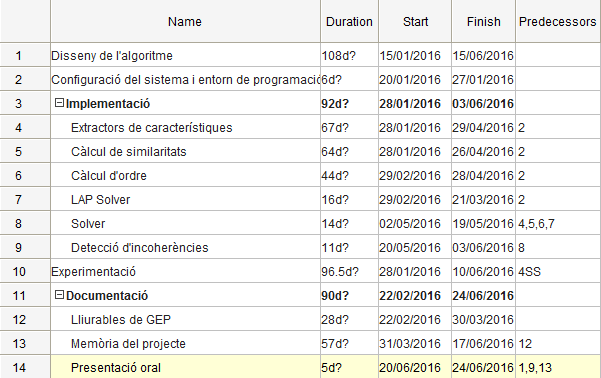
\includegraphics[width=\textwidth]{figures/gantt1.png}
    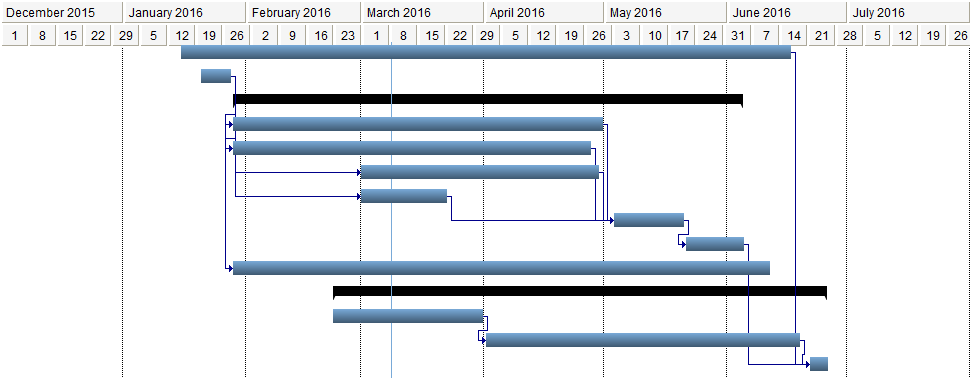
\includegraphics[width=\textwidth]{figures/gantt2.png}
    \caption{El diagrama de gantt de la planificació temporal del projecte abans de la realització.}
    \label{fig:gantt}
\end{figure}

\begin{figure}[!htb]
    \centering
    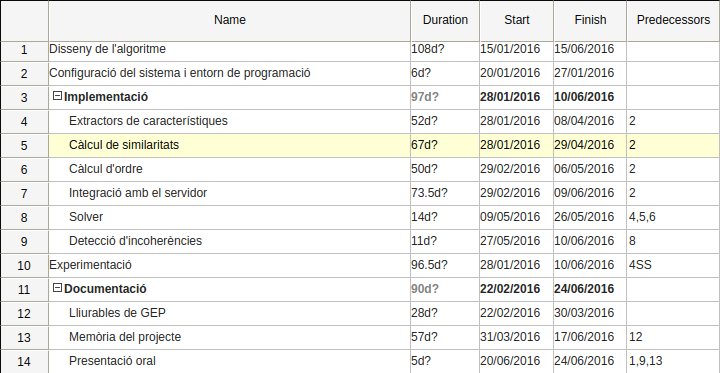
\includegraphics[width=\textwidth]{figures/gantt2_1.png}
    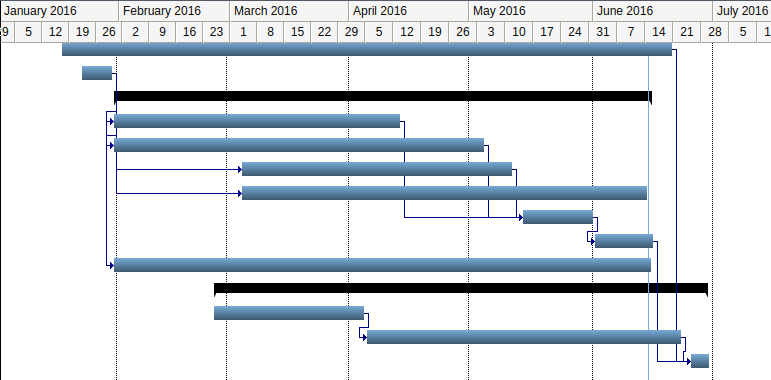
\includegraphics[width=\textwidth]{figures/gantt2_2.png}
    \caption{El diagrama de gantt que reflexa l'evolució real que ha tingut el projecte.}
    \label{fig:gantt}
\end{figure}

\clearpage

\subsection{Pla d'acció inicial i desviacions}

El pla d'acció inicial ha consistit en dur a terme les tasques planejades tal com estaven especificades al diagrama de Gantt de la fita inicial. No obstant això, s'ha de tenir en compte que aquest és un projecte amb un fort component exploratori. Així doncs, a priori, podia semblar això que pot resultar difícil adaptar-se al pla dissenyat. Una decisió de disseny provinent de nous fets que surten fruit de l'experimentació pot fer que algun dels mòduls de l'algorisme deixi de ser necessari o necessiti canvis substancials. Veiem doncs com és probable que aquesta planificació evolucioni al llarg del projecte.

L'objectiu del projecte és clar: Tenir un algorisme que funcioni per a resoldre el problema descrit. Tot i això inicialment hi havia moltes parts en les quals hi havia molt poc decidit i on resultava difícil fer una estimació raonable d'hores. L'eina principal de control de temps ha estat la quantitat d'exploració en les diferents parts de l'algorisme. 

El primer lloc on trobem molta flexibilitat és en la quantitat de característiques que s'extreuen del text i el model. Com més tipus de característiques s'explorin més qualitat tindrà l'algorisme\footnote{Aixo no vol dir que l'algorisme final faci l'extracció de totes les característiques implementades. Ans al contrari, com més d'aquestes es plantegin i s'avaluin més informat serà l'algorisme i per tant, en general, millor.}. Inicialment s'havia plantejat que, en cas de falta de temps es podria optar per explorar menys tipus de característiques a extreure. Finalment, el conjunt de característiques que s'han explorat ha estat prou gran, i dóna uns resultats bastant satisfactoris.

Un altre punt que ens permet ajustar el temps final de desenvolupament és la quantitat d'experimentació. Com més alternatives s'explorin quant a mètriques de similaritat i algorismes d'optimització millor serà l'algorisme final. El punt on s'ha invertit més temps d'experimentació ha estat en el càlcul de l'assignació òptima, la tasca del Solver. Això ha fet que s'hagués de retallar temps de l'exploració de diferents mètriques de similaritat.

Finalment, la tasca d'intentar reduir el problema a un LAP, per veure si la solució obtinguda és una bona aproximació, s'havia considerat com opcional. No obstant això finalment s'ha pogut explorar l'opció i implementar-la.

Com es pot veure a la taula de temps. La quantitat d'hores prevista per completar aquest projecte és de 530 hores, que coincideix amb les hores per crèdit orientatives establertes a la normativa del treball de final de grau a la FIB. Tenint en compte que la durada del projecte ha estat de 24 setmanes aproximadament, podem veure que la dedicació mitjana ha estat de 22,5 hores per setmana, que descomptant dos dies per setmana equival a 4,5 hores de treball diàries. Veiem que és una quantitat d'hores viable.


\section{Pressupost}
\label{pressupost}

En aquesta secció es fa un anàlisi detallat dels costos per a la realització d'aquest TFG. Els diferents apartats corresponen als diferents tipus de despeses que es plantegen. 

Cal tenir en compte que aquest pressupost s'ha dissenyat com si es tractés d'un projecte d'enginyeria en una empresa real, i que no tots els costos --Especialment els referents als recursos humans-- reflecteixen la realitat del projecte.

\subsection{Recursos humans}

La major part de tasques d'aquest projecte corresponen a una sola persona\footnote{Tret de la tasca de disseny de l'algorisme, que es realitza de manera conjunta entre l'alumne i els directors de projecte.}. Aquest, però, no seria el cas en un projecte real. A l'hora de fer aquest pressupost s'han tingut en compte els diferents rols que intervindrien en un projecte similar. Així doncs, els recursos humans s'han dividit en els rols de: Cap de projecte, dissenyador, programador, \emph{beta tester} i documentador.

Tenint en compte les diferents tasques definides a la planificació temporal, podem estimar les hores de cadascun dels membres de l'equip:

\begin{itemize}
    \item La configuració de l'entorn de programació correspondria al programador, que és qui estableix els requisits de l'entorn. (15h)
    \item El disseny de l'algorisme correspondria conjuntament al Cap de projecte i al Dissenyador. El temps planejat de la part de disseny no es parteix, és simultani\footnote{És important notar aquest fet, ja que fa que les hores del pressupost no sumin el mateix que les hores totals del projecte.}. (90+90h)
    \item La implementació de l'algorisme corresponen al programador i al \emph{beta tester}. El temps total es reparteix entre els dos rols. (180+70h)
    \item L'experimentació correspon al dissenyador, encarregat de dissenyar els experiments. Es comptabilitzen també unes hores del programador per implementar el codi dels experiments. (75+10h)
    \item La documentació correspon al rol de documentador. (100h)
\end{itemize}

A la taula \ref{tab:recursos_humans} es pot veure el pressupost estimat considerant un sou adequat per cadascun dels rols.

\begin{table}[!htb]
    \centering
    \begin{tabular}{|l||c|r|r|}
        \hline
         Rol & Preu per hora & Hores & Cost \\
         \hline\hline
         Cap de projecte & 50.00€/h & 90h & 4500.00€ \\
         Dissenyador & 35.00€/h & 165h & 5775.00€ \\
         Programador & 30.00€/h & 190h & 5700.00€ \\
         \emph{Beta tester} & 30.00€/h & 70h & 2100.00€ \\
         Documentador & 30.00€/h & 100h & 3000.00€ \\
         \hline\hline
         TOTAL & & & 21075.00€ \\
         \hline
    \end{tabular}
    \caption{Estimació del pressupost dels recursos humans.}
    \label{tab:recursos_humans}
\end{table}

\subsection{Recursos de hardware}

A la taula \ref{tab:recursos_hardware} es descriu el pressupost que s'ha estimat per als recursos de hardware necessaris per dur a terme el projecte. La falta de dades sobre les màquines del \emph{Textserver} fa que no en puguem estimar un pressupost. D'altra banda res impedeix instal·lar \emph{Freeling} en local i executar-lo en la mateixa màquina amb la qual es desenvolupa el projecte si el servidor suposés un cost important.

\begin{table}[]
    \centering
    \begin{tabular}{|l||r|c|r|}
        \hline
         Producte & Preu & Vida útil & Amortització \\
         \hline\hline
         Ordinador portàtil & 700.00€ & 4 anys & 50.00€ \\
         Màquines del \emph{Textserver} & 0.00€ & desconegut & 0.00€ \\
         \hline\hline
         TOTAL & 700.00€ & & 50.00€ \\
         \hline
    \end{tabular}
    \caption{Estimació del pressupost dels recursos de software.}
    \label{tab:recursos_hardware}
\end{table}

\subsection{Recursos de software}

A la taula \ref{tab:recursos_software} es descriu el pressupost estimat per als recursos de software del projecte. Com es pot observar el pressupost és purament un formalisme, ja que tots els recursos de software utilitzats són totalment gratuïts.

\begin{table}[!htb]
    \centering
    \begin{tabular}{|l||c|c|r|}
        \hline
         Producte & Preu & Vida útil & Amortització \\
         \hline\hline
         Freeling & 0.00€ & -- & 0.00€ \\
         Activiti & 0.00€ & -- & 0.00€ \\
         Arch GNU/Linux & 0.00€ & -- & 0.00€ \\
         Clojure & 0.00€ & -- & 0.00€ \\
         Java & 0.00€ & -- & 0.00€ \\
         Maven & 0.00€ & -- & 0.00€ \\
         \LaTeX & 0.00€ & -- & 0.00€ \\
         Gannter & 0.00€ & -- & 0.00€ \\
         \hline\hline
         TOTAL & & & 0.00€ \\
         \hline
    \end{tabular}
    \caption{Estimació del pressupost dels recursos de software.}
    \label{tab:recursos_software}
\end{table}


\subsection{Despeses indirectes}

Les despeses indirectes tenen en compte l'ús d'electricitat i material d'oficina necessaris per a la realització d'aquest projecte. La taula \ref{tab:recursos_indirectes} mostra una estimació del pressupost d'aquestes despeses.

El preu de l'electricitat s'ha calculat tenint en compte el preu del $KW/h$ a la ciutat de Barcelona i les hores del projecte en les que, segons la planificació, és necessari l'ús de l'ordinador\footnote{L'ordinador consumeix 120W, com es comenta a l'apartat de recursos.}. A més, s'inclou una part addicional en previsió de la llum necessària per desenvolupar el projecte.

Pel que fa al material d'oficina s'ha escollit un preu raonable per tal que la falta de material no resulti un inconvenient. Cal destacar que aquest projecte no en requereix un ús intensiu.

\begin{table}[!htb]
    \centering
    \begin{tabular}{|l||c|c|r|}
        \hline
         Producte & Preu & Unitats & Cost \\
         \hline\hline
         Electricitat (portatil) & 0.141€/KWh & 54Kwh\footnote{Connectat a la corrent sense bateria amb un transformador de 19V i 6.32A (120W).} & 7.61€\\
         \hline\hline
         Electricitat (llum) & 0.141€/KWh & 20Kwh\footnote{Dues bombetes de baix consum (15W)} & 7.61€\\
         \hline\hline
         Material d'oficina & 25.00€/unitat & 1 & 25.00€ \\
         \hline\hline
         TOTAL & & & 32.61€ \\
         \hline
    \end{tabular}
    \caption{Estimació del pressupost dels recursos indirectes.}
    \label{tab:recursos_indirectes}
\end{table}


\subsection{Pressupost total}

A la taula \ref{tab:total} es mostra el pressupost global del projecte, on es pot veure que la part que aporta més al cost del projecte és la dels recursos humans. A l'apartat \ref{economica} es realitza la valoració global d'aquest pressupost.

\begin{table}[!htb]
    \centering
    \begin{tabular}{|l|r|}
        \hline
         Concepte & Preu \\
         \hline\hline
         Recursos Humans & 21075.00€ \\
         Recursos de Software & 0.00€ \\
         Recursos de Hardware & 50.00€ \\
         Despeses indirectes & 32.61€ \\
         \hline\hline
         TOTAL & 21157.61€ \\
         \hline
    \end{tabular}
    \caption{Estimació del pressupost total.}
    \label{tab:total}
\end{table}

\subsection{Control de gestió}
\label{control}

En aquesta secció es considera com podria modificar-se aquest pressupost davant d'imprevistos i es proposen alternatives per tal de compensar-ho.

Com es veu a l'apartat anterior, pràcticament la totalitat del cost del projecte correspon als recursos humans. És per aquest fet que possibles desviacions en la planificació temporal poden afectar molt significativament al pressupost del projecte. Si es dóna el cas, cal sospesar si és més profitós reduir funcionalitats del projecte final o augmentar les hores totals del projecte. El primer escenari possiblement comportarà menys beneficis donat que s'haurà obtingut un producte de menys qualitat, mentre que amb el segon pot augmentar considerablement el pressupost final.

Pel que fa al software, un possible imprevist seria la incorporació de codi amb llicències de pagament en el projecte. En cas de ser inevitable s'haurà d'assumir el cost però sempre que sigui possible s'optarà per alternatives gratuïtes i, si és possible, de codi obert.

Pel que fa al hardware i al consum elèctric no es preveuen desviacions. Realment l'únic necessari per implementar l'algorisme és un ordinador i algun material complementari (papers, bolígrafs, etc.).



\section{Informe de sostenibilitat}

En aquesta secció s'inclou l'anàlisi de sostenibilitat feta per aquest projecte. En primer lloc es presenta la matriu de sostenibilitat del projecte i posteriorment se'n realitza una anàlisi per files justificant les puntuacions assignades a cada casella de la matriu.

\subsection{Matriu de sostenibilitat}
La taula \ref{tab:matriu_sostenibilitat} mostra la matriu de sostenibilitat d'aquest projecte. La puntuació de sostenibilitat total del projecte és de 70 punts, el que ens indica que és un projecte suficientment viable i sostenible.
\begin{table}[!htb]
    \centering
    \begin{tabular}{|c|c|c|c|}
    \hline
         & PPP & Vida útil & Riscos \\
         \hline\hline
        Ambiental & 10 & 19 & 0 \\
        \hline
        Econòmic & 8 & 15 & -12 \\
        \hline
        Social & 10 & 8 & -5 \\
        \hline\hline
        Puntuació & 28 & 42  & -17\\
        \hline
        \textbf{Total} & \multicolumn{3}{c|}{70} \\
        \hline
    \end{tabular}
    \caption{Matriu de sostenibilitat}
    \label{tab:matriu_sostenibilitat}
\end{table}

\subsubsection{Dimensió ambiental}

Aquest projecte no requereix l'ús de manera directa de cap agent contaminant. L'únic necessari per al desenvolupament de l'algorisme és un ordinador, i el producte final és software. Tot i això l'ús d'energia elèctrica i aparells electrònics comporta, indirectament, l'emissió de gasos contaminants a l'atmosfera. Fent una estimació\footnote{S'ha utilitzat la calculadora d'emissions de CO2 disponible a: \url{http://arboliza.es/compensar-co2/calculo-co2.html}} del $CO_2$ emès, es calcula que el desenvolupament d'aquest projecte comportarà l'emissió de 48.1Kg de $CO_2$ alliberats a l'atmosfera. És important destacar que la utilització d'un ordinador portàtil com a eina principal de desenvolupament fa que el consum energètic sigui considerablement inferior que si s'hagués utilitzat un ordinador de sobretaula\footnote{Un ordinador de sobretaula equivalent consumiria uns 400W de mitjana en comptes dels 120W que gasta el portàtil.}. En tot cas, la quantitat de $CO_2$ generada per aquest projecte és molt inferior a la que genera una persona en els 6 mesos de durada d'aquest. Per aquest fet, s'ha donat la puntuació màxima de 10 punts a la casella Ambiental/PPP de la matriu.

Si aquest projecte s'acaba convertint en un software exitós, és probable que moltes empreses l'incorporin en els seus servidors i l'utilitzin de manera extensiva. És difícil estimar el consum energètic que això comportarà, però és innegable que un software executant-se contínuament en els servidors d'una empresa i que fa servir algorismes costosos té un cost energètic no negligible. D'altra banda, aquest fet es veuria possiblement compensat per l'estalvi de paper i material que suposaria l'automatització de totes les tasques relacionades amb el \emph{Business Process Management}. És per aquest fet que s'ha donat una puntuació de 19 a la casella Ambiental/Vida útil de la matriu de sostenibilitat. 

Finalment, cal comentar que no es preveu cap escenari en el qual aquest projecte pugui augmentar la seva petjada ecològica més enllà del que ja s'ha comentat en aquest document. És per això que s'assigna una puntuació de 0 a la casella Ambiental/Riscos.


\subsubsection{Dimensió econòmica}
\label{economica}

A l'apartat \ref{pressupost} ja es realitza una anàlisi detallat de tots els costos que intervenen en aquest projecte, tant humans com materials. Cal tenir en compte, però, que aquest és le pressupost de realització del projecte l'objectiu del qual és crear un software. El software resultant molt probablement requereixi manteniment, actualitzacions i expansions. 

És difícil reduir costos durant la realització del projecte. Quasi tot el cost del projecte recau en el cost dels sous dels desenvolupadors i les hores vénen marcades per la planificació temporal. No obstant una planificació més compacta i no tan centrada en l'experimentació podria ajudar a millorar en l'àmbit econòmic. El fet que aquest projecte aborda un problema que gairebé no s'ha tractat fins al moment a la literatura fa que sigui molt difícil parlar de reaprofitar codi per l'algorisme. A part, el cost tant en software com hardware és el mínim necessari. Per tot això s'assigna una puntuació de 8 a la casella Econòmic/PPP.

L'objectiu del projecte global és comercialitzar el producte resultant a empreses\footnote{Cal recordar que l'objectiu d'aquest TFG és l'algorisme que es desenvolupa en aquest TFG passi a formar part d'un paquet software que pugui servir per a les empreses centrades en \emph{Business Process Management}. Em refereixo a això amb el projecte global.}. La viabilitat econòmica d'aquest paquet de software depèn del model de distribució que s'esculli per comercialitzar-lo. Per una banda es pot optar per una llicència tancada i de pagament. Una possible alternativa a la venda per llicència, és un model de doble llicència: S'ofereix una versió bàsica del producte com a software gratuït perquè qualsevol empresa el pugui provar i es cobra per la versió completa, que permet l'ús del software per a mitjans comercials. És difícil determinar a priori el potencial de vendes del producte resultant, però si l'algorisme genera bons resultats, pot arribar a ser una eina de gran valor per a empreses centrades en el BPM. És per això que s'ha donat una puntuació de 16 a la casella Econòmic/Vida útil.

Si l'enfoc del tractament automàtic del \emph{Business Process Management} resulta profitós a les empreses centrades en aquesta pràctica, és molt probable que apareguin tot tipus de competidors al software d'aquest projecte. No obstant cal tenir en compte que s'estaria partint d'una posició avantatjosa, ja que aquest seria el primer software al mercat a oferir funcionalitats similars. És doncs important tenir en compte aquest risc a l'hora de comercialitzar el software final i per això s'ha donat una puntuació de -12 a la casella Econòmic/Riscos.

\subsubsection{Dimensió social}

Aquesta és, potser, la dimensió més rellevant per aquest projecte. Tant en aspectes positius com també en negatius.

Pels actors implicats en el desenvolupament d'aquest projecte, el desenvolupament d'aquest comporta un creixement personal. Concretament, com a alumne, m'acosta al món de la recerca, i em dóna una bona visió de l'algorítmia en un entorn pràctic i realista com és el \emph{Business Process Management} en combinació amb el \emph{Natural Language Processing}. A part, el fort component de programació del projecte i l'elecció de les eines de treball em comporta un creixement personal especialment com a programador. A més d'haver treballat en un projecte gran i amb utilitat pràctica directa per primera vegada. És per això que he puntuat amb un 10 la casella Social/PPP de la matriu.

La documentació i anàlisi dels processos de negoci en empreses resulta una manera molt bona de controlar les activitats d'una empresa de cara a optimitzar-ne el cost. És evident, doncs, que l'automatització d'aquestes tasques tindrà un impacte positiu directe en el rendiment econòmic de l'empresa. A més, l'algorisme desenvolupat en aquest TFG pot estalviar una gran quantitat d'hores de treball repetitiu assistint en la cerca d'incoherències entre els models BPMN i les seves representacions textuals. No obstant això, aquest mateix estalvi pot resultar en un impacte negatiu pel col·lectiu d'empleats que treballi desenvolupant aquestes mateixes tasques. Aquest últim fet es veuria especialment accentuat si les empreses decideixen retallar en la seva plantilla com a resultat de l'automatització d'aquesta tasca. És per això que s'assigna una puntuació de 15 a la casella Social/Vida útil de la matriu de sostenibilitat.

Com ja s'ha comentat, la pèrdua de llocs de treball fruit de l'automatització de les tasques en les quals assisteix l'algorisme d'aquest projecte pot ser vista com un risc per a la gent que treballa en aquest tipus de feines. No obstant s'ha de tenir en compte que això també pot ser vist com una oportunitat de reassignar aquests treballadors en tasques de més alt nivell. A més, si el resultat d'aquest projecte comporta beneficis a una empresa aquesta té un major potencial de creació de llocs de treball. Hi han riscos, però es poden evitar. Per això s'assigna una puntuació de -5 a la casella Social/Riscos de la matriu de sostenibilitat.

\section{Metodologia i rigor}

En aquesta secció es descriu la metodologia emprada de cara a un correcte i fluid desenvolupament del projecte. 

\subsection{Metodologia de treball}

Tot i que els requisits del sistema a dissenyar, a grans trets, són relativament estàtics: ``Dissenyar un algorisme que resolgui un problema concret'', quan mirem les tasques a realitzar amb un nivell de granularitat més fina veiem que els requisits del projecte poden variar notablement. Les diferents eines que s'han utilitzat, i decidir com s'ha modelat el problema en els diferents punts de l'algorisme han produït canvis en la planificació per diversos motius: Ja sigui perquè s'ha trobat una idea millor, o perquè han aparegut nous angles al problema que fan que decisions que s'havien pres inicialment no encaixin del tot amb els nous requisits. És per això que aquest projecte s'ha desenvolupat seguint una metodologia de desenvolupament àgil \cite{agile_manifesto}.

El projecte s'ha desenvolupat amb iteracions d'una o dues setmanes. Al principi de cada iteració es planteja la llista de tasques a realitzar i al final es realitza una avaluació de la feina feta, replanificant adientment. La planificació i seguiment de les tasques es realitza utilitzant una taula \emph{Kanban}, que permet fer una planificació de tasques concretes a curt termini, acompanyada de la planificació general per tenir una visió de l'estat global. A més, es realitza un control estricte del temps durant les estones de treball inserint descansos periòdics per millorar la productivitat\footnote{Aquesta tècnica és coneguda com a \emph{timeboxing}.}.

\subsection{Eines de seguiment}

Cada setmana es fa una reunió de seguiment amb els directors del projecte, coincidint amb l'inici d'una nova iteració de desenvolupament. En les reunions, es mostren els resultats obtinguts, l'estat del projecte, i es plantegen tots els problemes o dubtes que han pogut aparèixer. A continuació, es fa una valoració de la feina realitzada respecte als objectius marcats a la setmana anterior. Finalment, es decideix la llista d'objectius a assolir per la setmana vinent: Funcionalitats del programa, possibles experiments, i/o documentació.

Tret de les reunions setmanals, la resta de comunicació s'ha fet per correu electrònic. L'objectiu és plantejar els temes importants com més aviat millor de cara a rebre \emph{feedback} ràpidament, i si escau, resoldre els problemes o dubtes abans de la següent reunió amb l'objectiu de fer avançar el projecte de manera fluida. 

Finalment, donat que aquest projecte forma part d'un projecte més gran de diferents alumnes treballant en l'àmbit de NLP per a BPM, amb menys freqüència, s'han fet reunions amb tots els membres amb l'objectiu d'agafar perspectiva en els projectes individuals de cadascú i per veure si hi ha alguna part comuna que es pugui compartir.

\subsection{Mètode de validació}

En el cas d'aquest projecte, la validació de resultats és una tasca complicada. Per analitzar la qualitat dels resultats obtinguts de manera objectiva i automàtica caldria una eina que resolgui el problema que es planteja resoldre aquest projecte. És per això que serà necessaria una validació manual.

Així doncs, per avaluar la qualitat de les solucions s'usarà un conjunt suficientment gran d'exemples diversos, alternant casos amb incoherències i sense incoherències. 

Com que la similaritat entre un model BPMN i un document escrit és difícil de determinar, caldrà recorrer a un expert\footnote{Els experts seràn en aquest cas els directors del projecte.} que corrobori els resultats per avaluar la qualitat del software final.

Sobre aquest conjunt de dades d'exemple podrem elaborar un estudi en funció dels resultats de l'algorisme fent servir diverses mètriques emprades en camps similars com són el \emph{recall} i la \emph{precision}.



\section{Integració de coneixements}
\label{integracio}
En aquesta secció es discuteixen les diferents disciplines de la informàtica que intervenen en aquest projecte en més o menys mesura i com hi estàn integrades.

Aquest projecte és una combinació de dues disciplines concretes de la informàtica. El \textit{Natural Language Processing} i el \textit{Business Process Management}. Els dos camps es troben en recerca activa i els resultats obtinguts en aquests utilitzen tot tipus de tècniques de diferents camps com la intel·ligència artificial, la teoria de grafs o l'algorísmia.

Per a l'elaboració del projecte s'utilitzen, o s'han plantejat utilitzar\footnote{No totes les alternatives plantejades han acabat al projecte original, però això no vol dir que no s'hagin estudiat i valorat.} les següents tècniques i algorismes relacionades amb els continguts de la carrera:

\begin{itemize}
\item Freeling, com a analitzador semàntic.
\item Solver de Constraint Programming.
\item Mètriques de distancia.
\item Vectors de característiques.
\item Similaritat semàntica en Wordnet.
\item Càlcul de Behavioral Profiles en grafs de processos.
\item Algorismes de grafs de flux, concretament el d'eliminació de back-edges.
\item Linear Assignment Problem i l'Hungarian Method.
\item Programació funcional.
\end{itemize}

\section{Lleis i regulacions}
\label{lleis}
En aquest apartat es fa una breu discussió de l'apartat legal rellevant en el marc del projecte.

Pel que fa al producte resultant, aquest és una eina que està planejada per assistir en tècniques de Business Process Management. Actualment no existeix cap legislació que reguli com una empresa ha de documentar els seus processos des d'un punt de vista de BPM, i si es requerís d'alguna documentació en un camp concret aquesta existeix separada de la documentació formal dels processos de negoci. Així doncs podem dir que no hi ha cap normativa que s'hagi de tenir en compte a l'hora de parlar del producte resultant.

No obstant, pel que fa al desenvolupament del software i les opcions de comercialització, cal tenir en compte quines són les llicències utilitzades en totes les llibreries que aquest integra, i quina serà la llicència del producte final. S'ha d'anar en compte amb no incumplir cap dels termes i condicions de totes les llicències que s'estàn fent servir. 


